\documentclass[a4paper, 12pt]{article}

% include required packages
\usepackage[a4paper, margin=2cm]{geometry} % Set page margins
\usepackage[round,authoryear]{natbib}      % For citations
\usepackage{url}                           % For formatting URLs
\usepackage{indentfirst}                   % Indent first paragraph of sections
\usepackage{booktabs}                      % For better table formatting
\usepackage{float}                         % For [H] table placement
\usepackage{enumitem}                      % For customizing lists
\usepackage{tikz}                          % For drawing diagrams
\usetikzlibrary{positioning}               % For relative positioning

% set paragraph and list formatting
\setlength{\parindent}{1.5em}
\setlength{\parskip}{0pt}
\setlist[itemize]{noitemsep,topsep=0pt,parsep=0pt,partopsep=0pt,after=\vspace{0.5em}}


% set title information
\title{Incorporating usability and user experience into the Web Witchcraft and Wizardry project}
\author{Edmund Mulligan}
\date{\today}

% document start
\begin{document}

% set bibliography style and page numbering
\bibliographystyle{plainnat}
\pagenumbering{arabic}

\maketitle

\begin{abstract}
\textit{The application of WCAG 2.2 and Nielsen's usability heuristics are considered in relation to a website redesign aimed at teaching 
web development concepts and skills to children. The specific needs of the target audience are discussed and classified using the WCA guidelines.
A metaphor based on popular fantasy literature is proposed to engage young learners. The use of automation tools in the development and deployment 
process is considered as a means of ensuring ongoing usability and accessibility compliance.}
\end{abstract}

\section*{Introduction}

Web Witchcraft and Wizardry \citep{mulligan2024witchcraftandwizardry} is a project developed for Kingston University Code 
Dojo to teach web development concepts and skills to beginners, specifically children aged between about 8 and 15 years who have some 
experience of developing games and applications using block-based programming languages such as Scratch \citep{resnick2009scratch} and Blockly 
\citep{bau2017learnable}. Learners are supported by adult mentors, who may have limited experience of web development themselves. Clearly, 
publishing this project on the World Wide Web opens it to a much wider audience, but also raises important usability and user experience (UX) 
considerations that must be addressed to ensure the project is effective in achieving its educational goals \citep{kafai2014connected}. 

This essay reviews how the Web Content Accessibility (WCA) Guidelines \citep{caldwell2024} apply in the context of the specific target audience 
for the project. It also considers Nielsen's \citep{nielsen1994enhancing, neilsen2024usability} heuristics, although Nielsen is focused on usability 
rather than the accessibility of WCAG 2.2 \citep{petrie2007relationship}. Together they provide a framework for evaluating usability and accessibility 
and this essay discusses how UX design principles can be incorporated into the project to enhance learner engagement and satisfaction. 

Not all guidelines and heuristics are equally relevant to any project, and the specific characteristics of young learners and their adult mentors 
must be taken into account when applying these principles. As the scope of the assessment of this project is limited to a few web pages, 
consideration of the user experience for mentors is not included in this essay, although it is acknowledged that this is an important aspect of 
the overall user experience. The essay concludes with recommendations for further work to evaluate and improve the usability and UX of the Web 
Witchcraft and Wizardry project.

\section*{Inclusivity and accessibility}

While the project is primarily targeted at young learners, it is important to consider inclusivity and accessibility to ensure that all users, 
regardless of their abilities or backgrounds, can benefit from the educational content. The WCA guidelines provide a comprehensive framework 
for designing accessible web content, summarised as five principles in table~\ref{tab:wcag-principles}, although the fifth is not relevant 
here as the website will not be formally asserting its conformance to WCAG 2.2.
\begin{table}[H]
\centering
\begin{tabular}{lp{10cm}}
\toprule
\textbf{Principle} & \textbf{Description} \\
\midrule
1. Perceivable & Users need to be able to perceive the content \\
2. Operable & All users need to be able to operate the interface \\
3. Understandable & Users need to be able to understand information and UI operation \\
4. Robust & The content must work with assistive technologies \\
5. Conformance & An optional principle used when asserting a web page meets WCAG standards \\
\bottomrule
\end{tabular}
\caption{WCAG 2.2 Accessibility Principles}\label{tab:wcag-principles}
\end{table}

In addition to general considerations, the specific needs of young learners must be addressed \citep{druin2002role}. This means 
taking account of the cognitive and reading abilities of children by providing appropriate scaffolding \citep{wood1976role}, and suitable 
metaphors \citep{vosniadou1989analogical, bau2017learnable}. Some of these requirements relate to the visual appearance of the web content, 
such as the use of engaging images and colours. While these aspects are important, they are best left until phase 2 of the project which focuses 
on visual design aesthetics. Other requirements fall within the scope of this essay such as having simple, consistent navigation with clear 
labels and visual cues, minimising the cognitive load by breaking complex concepts into small, digestible chunks and providing immediate, 
positive feedback for interactions.

Users of the website are, of course,  free to use whatever devices they choose, but as it is teaching web development, it is assumed that they 
will have access to a computer capable of running the development tools required in the lessons. This means that considerations such as small 
screen sizes and touch-only input are less relevant, although the website will be designed to be responsive should they want to use a mobile 
device alongside the computer.

\section*{An age appropriate design for teaching web development}

Many, perhaps most, children within the target age range for the Web Witchcraft and Wizardry project are familiar with the Harry Potter series of 
books and films \citep{rowling1997series}, which provides a rich source of metaphors for explaining programming concepts. For example, 
the idea of casting spells can be used to illustrate the concept of functions in programming. An alternative metaphor can be derived from the 
wizards and witches in Terry Pratchett's Discworld series \citep{pratchett1983discworld}, who often use magic in a humorous and unconventional 
way. Pratchett's work also provides a sound pedagogic model is the form of ``lies to children'' \citep{pratchett1999science}, where fictional 
elements and simplifications are used to engage children's imaginations while introducing them to real scientific concepts. By leveraging familiar 
metaphors, scaffolding \citep{wood1976role} can be constructed to support children's understanding of web development concepts in a fun and 
engaging way.

This essay does not discuss the detailed information architecture of the website, but to give a brief overview, the content is organised into a 
series of lessons, each focusing on a specific web development concept or skill. A proposed navigation structure is shown in 
figure~\ref{fig:site-map}, which can be referred to when considering the application of WCAG guidelines and Nielsen's heuristics.

\begin{figure}[H]
\centering
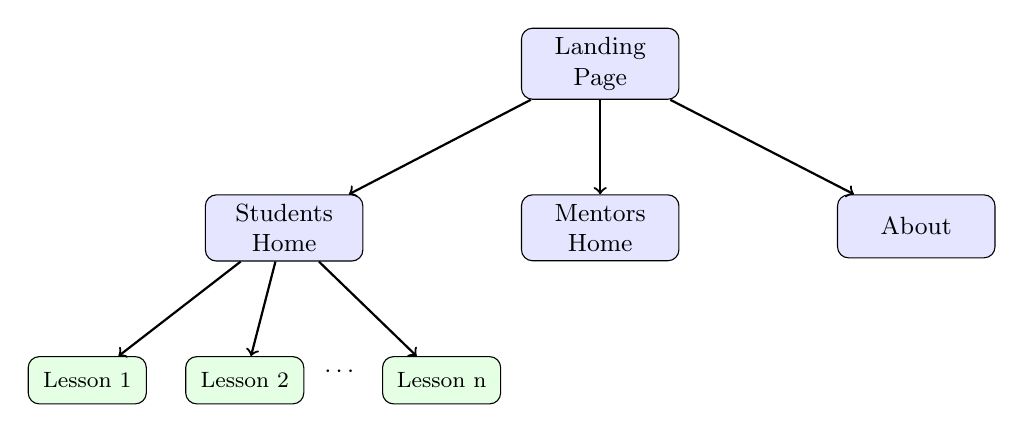
\begin{tikzpicture}[
  node distance=1.2cm and 1.5cm,
  box/.style={rectangle, draw, rounded corners, minimum width=2cm, minimum height=0.8cm, align=center, fill=blue!10, font=\small},
  lesson/.style={rectangle, draw, rounded corners, minimum width=1.5cm, minimum height=0.6cm, align=center, fill=green!10, font=\footnotesize},
  arrow/.style={->, thick}
]

% Top level - Landing Page
\node[box] (landing) {Landing\\Page};

% Second level - Main sections
\node[box, below left=of landing, xshift=-0.5cm] (students) {Students\\Home};
\node[box, below=of landing] (mentors) {Mentors\\Home};
\node[box, below right=of landing, xshift=0.5cm] (about) {About};

% Third level - Lesson pages under Students (arranged more compactly)
\node[lesson, below=of students, xshift=-2.5cm] (lesson-1) {Lesson 1};
\node[lesson, below=of students, xshift=-0.5cm] (lesson-2) {Lesson 2};
\node[lesson, below=of students, xshift=2cm] (lesson-n) {Lesson n};

% Ellipsis positioned between lesson 2 and lesson n
\node[below=of students, xshift=0.7cm] (dots) {\small $\cdots$};

% Arrows from Landing Page
\draw[arrow] (landing) -- (students);
\draw[arrow] (landing) -- (mentors);
\draw[arrow] (landing) -- (about);

% Arrows from Students Home to Lessons
\draw[arrow] (students) -- (lesson-1);
\draw[arrow] (students) -- (lesson-2);
\draw[arrow] (students) -- (lesson-n);

\end{tikzpicture}
\caption{Partial site map for Web Witchcraft and Wizardry project showing hierarchical navigation structure}\label{fig:site-map}
\end{figure}

The development methodology used in this project is also outside the scope of this essay, but to set the scope of 
work involved, an iterative approach will be used with the project divided into three phases:
\begin{itemize}
  \item Phase 1: A minimal viable product conformant to WCAG 2.2 level AA (Winter 2025)
  \item Phase 2: Visual design and aesthetics (Spring 2026)
  \item Phase 3: Full implementation and deployment (After PG Diploma completion)
\end{itemize}

Having established a suitable metaphor and information architecture for the intended users, specific WCAG guidelines can be applied to
ensure the web content is accessible and usable. This enumeration is necessarily brief, but highlights the most important features that need to
be considered for the project. Where there is overlap, Nielsen's heuristics (numbered N1 to N10) are also noted, but for reasons of space,
these are not elaborated in detail.

\subsection*{WCAG 1.1 Text Alternatives}

This guideline ensures that all users, including those with visual impairments, can access the content. It will be met by 
providing appropriate alternative text for images and other non-text content.

\subsection*{WCAG 1.2 Time-based Media}

This guideline is not relevant to this project, which will not include video or audio (time-based) content.

\subsection*{WCAG 1.3 Adaptable}

The website will be designed to work in both landscape and portrait mode, using responsive CSS techniques. This will ensure that the content is 
accessible on a variety of devices, including tablets and smartphones, which are increasingly used for web browsing. All instructions and lessons 
will, at a minimum, be in text format to ensure compatibility with screen readers and other assistive technologies.

\subsection*{WCAG 1.4 Distinguishable}

\begin{itemize}
  \item N8 Aesthetic and minimalist design
\end{itemize}

This important guideline will be considered more fully in phase 2 of the project, which focuses on visual design aesthetics. 

\subsection*{WCAG 2.1 Keyboard Accessible}

\begin{itemize}
  \item N3 User control and freedom
  \item N7 Flexibility and efficiency of use 
\end{itemize}

Keyboard navigation will be provided throughout the lessons and the website will be tested both with and without using a mouse.

\subsection*{WCAG 2.2 Enough Time}
\begin{itemize}
  \item N1 Visibility of System Status
  \item N2 User control and freedom
\end{itemize}

There will be no time limits used in any exercises. Users will be able to browse and navigate the site at their own pace.

\subsection*{WCAG 2.3 Seizures and Physical Reactions}

Flashing will not be used as an alert and any animation used will be able to be disabled by the user.

\subsection*{WCAG 2.4 Navigable}

\begin{itemize}
  \item N1 Visibility of System Status
  \item N6 Recognition rather than recall
  \item N7 Flexibility and efficiency of use
\end{itemize}

All web pages will have descriptive titles and make use of semantic HTML5 elements to ensure users can easily find their way around the site. 
A consistent layout for each lesson will be used throughout the site to aid navigation.

\subsection*{WCAG 2.5 Input Modalities}

At a minimum, the website will support input using a mouse, a keyboard and touch screen. Use of voice recognition may be considered in future,
but is not a priority at this stage. Other technologies such as motion capture will not be supported.

\subsection*{WCAG 3.1 Readable}

\begin{itemize}
  \item N2 Match between system and the real world
\end{itemize}

The site will only use the English language and this will be recorded in the web pages' metadata. A glossary will be developed to assist 
those new to programming concepts to easily understand unfamiliar terms, and abbreviations, unless in common usage, will be avoided or 
defined. The Flesch-Kincaid readability test \citep{kincaid1948new} will be used to ensure the text is appropriate for the target 
age range.

\subsection*{WCAG 3.2 Predictable}

\begin{itemize}
  \item N4 Consistency and standards
\end{itemize}

Navigation will be consistent throughout the site, with common elements such as menus and buttons appearing in the same location on each 
page, defined in one place and included where required. A consistent naming strategy will be used for lessons and other content.

\subsection*{WCAG 3.3 Input Assistance}

\begin{itemize}
  \item N5 Error prevention
  \item N6 Recognition rather than recall
  \item N9 Help users recognise, diagnose, and recover from errors
  \item N10 Help and documentation
\end{itemize}

Making mistakes is an important part of learning \citep{metcalfe2017learning, brown2014novice}, however it is also 
important that learners are not put off by intimidating error messages. Dropdown menus and other input controls 
will be used to minimise the risk of navigation errors (as opposed to expected coding errors) and clear, age-appropriate 
error messages will be provided to help users recover from mistakes. Errors generated by coding tools cannot be controlled, 
but where these can be predicted, explanations and suggestions for fixing common mistakes will be provided.

\subsection*{WCAG 4.1 Compatible}

Although access to assistive technologies is limited in this project, the website will be developed using 
semantic HTML5 elements to ensure compatibility with a wide range of devices and browsers, including screen 
readers.

\section*{Measuring and testing usability and the user experience}
To many non-technical people, usability and the user experience are qualitative (and hence unmeasurable) terms \citep{tractinsky2000}. In order 
to transcend this perception, the WCA principles are elaborated into guidelines with specific success criteria that can be tested and measured, making 
them a superior framework to Nielsen's heuristics which lack such metrics. WCAG 2.2 specifies three levels of conformance (A, AA and AAA) with an 
expectation that a website that meets all level A and AA success criteria will be generally accessible. But the WCA guidelines being testable is only 
useful if the website is actually tested. Manual testing of any sort, and particularly usability testing with real users, is time-consuming and 
expensive \citep{myers2011art}, so it is unlikely to be feasible within the constraints of this project. Further, manual testing is highly 
error-prone \citep{kaner1999testing}, so an automated approach will be used. 

There are many automated tools for testing web accessibility, three of which are Axe \citep{axe2025}, WAVE 
\citep{wave2025} and Lighthouse \citep{lighthouse2025}. These tools can identify common accessibility issues, such as missing alternative text for 
images, insufficient colour contrast, and poor keyboard navigation. They also produce detailed reports including scoring the website against the  
WCAG criteria, which can be used to prioritise improvements in an iterative design and development process. 

Automated testing is not a silver bullet 
\citep{kaner1999testing}, but in the absence of resources for manual testing, it is pragmatic. The risk of a particular tool missing important issues 
can be mitigated by using multiple tools and cross-referencing their results. The precise details of the automation test setup are outside the scope 
of this essay, but will be documented in the project repository using well commented GitHub actions.

\section*{Conclusion}

The Web Witchcraft and Wizardry project aims to teach web development concepts and skills to young learners using a fantasy metaphor to engage 
their imaginations. To ensure the project is effective, it is essential to consider usability and user experience principles, particularly those 
outlined in the WCAG 2.2 guidelines. By applying these principles, the project can create an inclusive and accessible learning environment for all 
users. Automated testing tools can be used to evaluate the website's accessibility and usability, providing a practical means of ensuring  
compliance during development and after deployment. Future work should focus on implementing the recommendations outlined in this essay, developing 
the visual aesthetics that have been not yet been considered, and conducting user testing with the target audience to gather feedback and further 
improve the user experience.

% Include word count N.B. Run wordcount.sh to generate wordcount.txt before compiling
\section*{Word count}
Word count: \input{wordcount.txt} words (excluding references)
\\
\bibliography{EdmundLibrary}

\end{document}
